%%%%%%%%%%%%%%%%%%%%%%%%%%%%%%%%%%%%%%%%%%%%%%%%%%%%%%%%%%%%%%%%%%%%%%%%%%%%%%%%%%%%%%%%%
%%                                                                                     %%
%%                This file is part of the CAPH Compiler distribution                  %%
%%                            http:%/caph.univ-bpclermont.fr                           %%
%%                                                                                     %%
%%                                  Jocelyn SEROT                                      %%
%%                         Jocelyn.Serot@univ-bpclermont.fr                            %%
%%                                                                                     %%
%%         Copyright 2011-2018 Jocelyn SEROT.  All rights reserved.                    %%
%%  This file is distributed under the terms of the GNU Library General Public License %%
%%      with the special exception on linking described in file ..%LICENSE.            %%
%%                                                                                     %%
%%%%%%%%%%%%%%%%%%%%%%%%%%%%%%%%%%%%%%%%%%%%%%%%%%%%%%%%%%%%%%%%%%%%%%%%%%%%%%%%%%%%%%%%%

\chapter{Dataflow programming}
\label{cha:lang-basic}

\caph is based upon a strict dataflow model of computation : Applications are described as networks
of computational units, called \emph{actors}, exchanging \emph{streams} of \emph{tokens} through
unidirectional, buffered channels. Data to be processed is simply ``pushed'' in the input ports of
the network and results are collected at output ports. Execution occurs as tokens litteraly ``flow''
through channels, into and out of actors.

\medskip This model of computation is illustrated on a very simple example in
Fig.~\ref{fig:networkfour}. The dataflow network operates on unstructured streams of tokens
carrying integer values. For each input token carrying value $x$, it produces a result
token carrying value $(x+1)\times(x-1)$. For instance, if the input stream (provided to the
\verb|dup| actor, through the \verb|i| input channel) is

\begin{verbatim}
1 2 3 4 ...
\end{verbatim}

the the output stream (produced by the \texttt{mul} actor, on the \verb|o| output channel) will be

\begin{verbatim}
0 3 8 15 ...
\end{verbatim}

\begin{figure}[h]
  \centering
  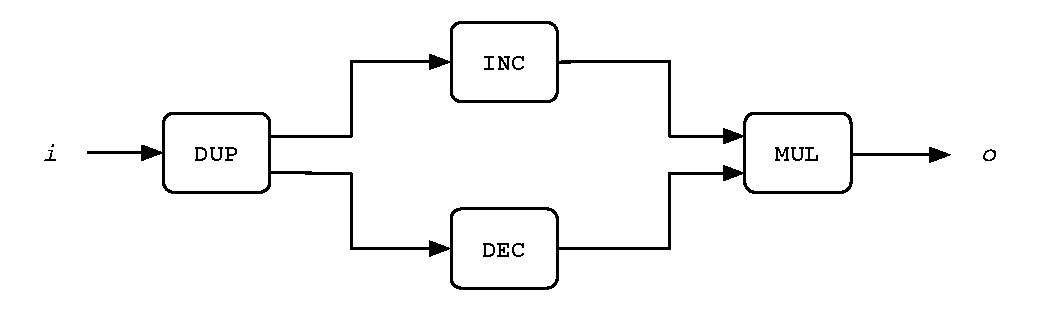
\includegraphics[width=0.75\textwidth]{figs/networkfour}
  \caption{A very simple dataflow network}
  \label{fig:networkfour}
\end{figure}

The network of Fig.~\ref{fig:networkfour} involves four simple actors. Actor \texttt{inc}
(resp. \texttt{inc}) adds (resp. substracts) 1 to each element of its input stream, actor
\texttt{mul} performs point-wise multiplication of two streams and actor \texttt{dup} duplicates its
input stream.

To understand what really ``happens'' when it is ``executed'' we need to attach a
\emph{semantics} both to actors and to the channels connecting these actors.

\medskip
The semantics of actors will be given as a set of \emph{firing rules} describing exactly \emph{when}
an actor executes (``fires'') and \emph{what} happens then. In this first example, the firing rule is the
same for each actor and it can be stated as : whenever a token is available on the channel connected
to each input port then read (``consume'') this token, compute the result(s) from the associated
value(s) and write (``produce'') the token(s) carrying this (these) result(s) on the channels
connected to the output port(s)\footnote{We will see latter that \caph allows more complex rules
  (and hence more sophisticated behaviors) to be expressed.}.

\medskip
The semantics of channels is simple : they will be viewed as FIFOs (First In First Out) buffers. In the
final implementation, the size of theses FIFOs will obviously be an important parameter. But for
now, let us consider that they are essentially unbounded.

\section{From sketch to code}
\label{sec:first-lines-code}

There's a long way from the rather ``informal'' description of an application as given in 
Fig.~\ref{fig:networkfour} to a FPGA configuration performing the described functionnality on a
stream of values.

The main steps in this path are illustrated in Fig.~\ref{fig:toolset}. These steps will be discussed
in part 2 and 3 of this document. Let's focus for the moment in the initial step, which is 
writing the source code of the application using the \caph language.

\begin{figure}[h]
  \centering
  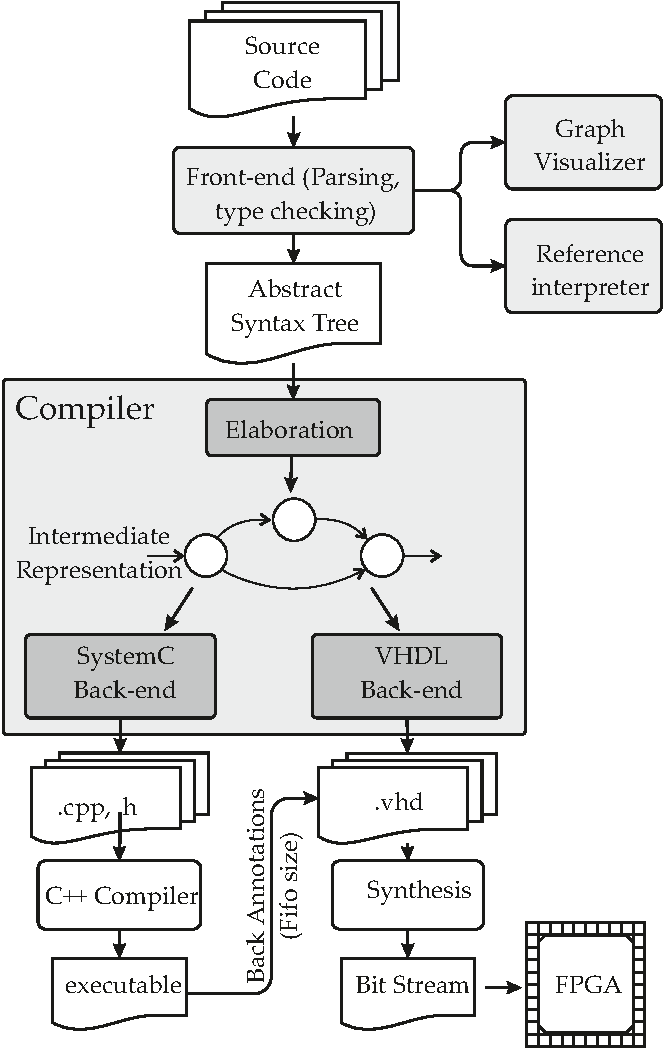
\includegraphics[width=0.4\textwidth]{figs/toolset}
  \caption{The CAPH design flow}
  \label{fig:toolset}
\end{figure}

\section{Writing the source code}
\label{sec:writing-source-code}

Let's write in \caph the description of the application depicted
in Fig.~\ref{fig:networkfour} in file \texttt{simple.cph}.

\medskip
We start by declaring the input and the output of the network :

\begin{lstlisting}[style=CaphStyle]
stream inp: unsigned<8> from "sample.txt";
stream outp: unsigned<8> to "result.txt";
\end{lstlisting}

The keyword \texttt{stream} introduces an I/O declaration. Each I/O has a name, a type and a
description. Here, we declare
\begin{itemize}
\item \texttt{inp} to be a input, with type \verb|unsigned<8>|, \emph{i.e.}
unsigned 8-bit integer, taking  values from a a file named \texttt{sample.txt}\footnote{As said
  above, this file will be used for simulation.}. 
\item \texttt{outp} to be an output, also with type \verb|unsigned<8>| putting values in a file
  named \texttt{result.txt}.
\end{itemize}

Concerning syntax, note that each declaration ends with a semi-colon.

\medskip
The next step consists in describing the network of actors. Basically, this involves specifying
which actors appear in this network and listing the connexions between these actor (``wiring'' the
network). In \caph\footnote{And for reasons which are advocated in the reference
  manual~\cite{caph-lrm}.}, this is done in a purely textual manner, by naming wires and viewing
actors as functions from wires to wires.

In this particular case, we start with the following declaration : 

\begin{lstlisting}[style=CaphStyle]
net (x1,x2) = dup inp;
\end{lstlisting}

This declaration, introduced by the \verb|net| keyword actually has two effects :
\begin{itemize}
\item first, it creates, in the network described by the program, a node named \texttt{dup},
\item second, it respectively \emph{binds} the input of this node to the wire named \emph{inp}
  (which, in this case is the input wire of the whole network) and  its outputs to two wires named
  \verb|x1| and \verb|x2|.
\end{itemize}

\medskip
We can now proceed (going ``from left to right'' in the graph of Fig.~\ref{fig:networkfour}), with
the following declarations : 

\begin{lstlisting}[style=CaphStyle]
net y1 = inc x1;
net y2 = dec x2;
\end{lstlisting}

The first declaration insert a nodes name \texttt{inc}, binding its 
input to the previously defined \texttt{x1} wire (\emph{i.e.} the first output of the \texttt{dup}
node) and its output to a new wire named \texttt{y1}. The second one does a similar thing with node
\texttt{dec} and wires \texttt{x2} and \texttt{y2} respectively.

\medskip
A last declaration inserts the \texttt{mul} node, connecting its inputs to the output of the
\texttt{inc} (resp. \texttt{dec}) node (by means of wires \texttt{y1} and \texttt{y2})  and its
output to the global output \texttt{outp} :

\begin{lstlisting}[style=CaphStyle]
net outp = mul (y1,y2);
\end{lstlisting}

\medskip
Note that the last three declarations could have been combined into a single one by writing :

\begin{lstlisting}[style=CaphStyle]
net outp = mul (inc x1, dec x2);
\end{lstlisting}

Which style is better -- with or without explicit naming of intermediate wires -- is essentially a
matter of taste since both will lead to exactly the same network. 

\medskip Together, the set of \texttt{stream} and \texttt{net} declarations introduced above
completely determines the \emph{static} stucture of the actor network\footnote{In other words, its
  \emph{topology}}.

\medskip
We now have to define the \emph{dynamic} behavior of the actors appearing in this network.

Let's start with the \texttt{inc} actor. Its behavior is specified by the following declaration :

\begin{lstlisting}[style=CaphStyle,numbers=left,numberstyle=\tiny]
actor inc
  in (i: unsigned<8>)
 out (o: unsigned<8>)
rules
| i:x -> o:x+1;
\end{lstlisting}

This declaration is composed of two parts : The first part (the \emph{interface}, lines 1--3) gives
the name of the actor and lists its inputs and outputs (giving a name and a type to each of them),
The second part (lines 4--5) specifies the behavior of the actor, by listing all the associated
firing rules. Here, there's only one rule\footnote{Each rule starts with a leading \texttt{|}.} and
it can be read as follows : whenever there's a token, carrying a value $x$, available on input
\texttt{i} then read (consumes) this token and write a token carrying value $x+1$ on output
\texttt{o}.

\medskip 
The definition of the \texttt{dec} actor is very similar : 

\begin{lstlisting}[style=CaphStyle]
actor dec
  in (i: unsigned<8>)
 out (o: unsigned<8>)
rules
| i:x -> o:x-1;
\end{lstlisting}

\medskip
The \texttt{mul} actor has two inputs and a single input. This is reflected in its interface and in
the format of the firing rule :

\begin{lstlisting}[style=CaphStyle]
actor mul
  in (i1: unsigned<8>, i2:unsigned<8>)
 out (o: unsigned<8>)
rules
| (i1:x, i2:y) -> o:x*y;
\end{lstlisting}

The interpretation of the firing rule for the \texttt{mul} actor is an obvious generalisation of the
one given for the two previous actors : the actor fires whenever a token (carrying values $x$ and
$y$ respectively) is available on \texttt{inputs}, \texttt{i1} and \texttt{i2}.  Concerning the
syntax, note the use of brackets on the left-hand side of the rule, which is mandatory here.

\medskip
The \texttt{dup} actor has a single input, but two outputs. This, again, is reflected in its
interface and the format of the firing rule :

\begin{lstlisting}[style=CaphStyle]
actor dup
  in (i: unsigned<8>)
 out (o1: unsigned<8>, o2:unsigned<8>)
rules
| i:x -> (o1:x, o2:x);
\end{lstlisting}

For this token, a token, carrying the same value ($x$) will be produced on both outputs
(\texttt{o1} and \texttt{o2}) whenever the actor fires.

\medskip
The full text of the program is given in Listing~\ref{lst:simple-full}. Note that, contrary to the
presentation order we have used above, the declarations of actors actually have to appear first
(this is because these declarations will be used by the \texttt{net} declarations). Comments are
introduced by the \verb|--| character sequence\footnote{Comments are single-line, like in Java.}. 

\begin{lstlisting}[style=CaphStyle,caption={Complete CAPH source code for the application
    depicted in Fig.~\ref{fig:networkfour}},label={lst:simple-full}]
-- Actor declarations

actor inc
  in (i: unsigned<8>)
 out (o: unsigned<8>)
rules
| i:x -> o:x+1;

actor dec
  in (i: unsigned<8>)
 out (o: unsigned<8>)
rules
| i:x -> o:x-1;

actor mul
  in (i1: unsigned<8>, i2:unsigned<8>)
 out (o: unsigned<8>)
rules
| (i1:x, i2:y) -> o:x*y;

actor dup
  in (i: unsigned<8>)
 out (o1: unsigned<8>, o2:unsigned<8>)
rules
| i:x -> (o1:x, o2:x);

-- I/O declarations

stream inp: unsigned<8> from "sample.txt";
stream outp: unsigned<8> to "result.txt";

-- Network declarations

net (x1,x2) = dup inp;
net y1 = inc x1;
net y2 = dec x2;
net outp = mul (y1,y2);
\end{lstlisting}

%%% Local Variables: 
%%% mode: latex
%%% TeX-master: "caph-primer"
%%% End: 
